\documentclass[11pt,a4paper]{article}

\usepackage[utf8]{inputenc}
\usepackage[T1]{fontenc}
\usepackage{amsmath,amssymb}
\usepackage{graphicx}
\usepackage{booktabs}
\usepackage{hyperref}
\usepackage[margin=0.9in]{geometry}
\usepackage{caption}
\usepackage{subcaption}
\usepackage{float}
\usepackage{xcolor}
\usepackage{array}

\newcommand{\etg}{$E_T$}
\newcommand{\crit}[1]{\textcolor{red}{\textbf{#1}}}
\newcommand{\fix}[1]{\textcolor[rgb]{0,0.5,0}{\textbf{#1}}}
\newcommand{\branch}[1]{\texttt{\small #1}}

\title{Isolation cone centering fix:\\
\large $|v_z|$-dependent mis-centering between cluster COG and tower centers,
and an ownership-excluded iso variant}
\author{PPG12 Analysis Team}
\date{April 18, 2026}

\begin{document}
\maketitle

\section*{Summary}

The manual tower-based and topo-cluster isolation computations in
\branch{anatreemaker/source/CaloAna24.cc} used \branch{RawClusterUtility::GetPseudorapidity(cluster, vertex)}
as the cone axis. That projects the cluster's stored position
(\branch{RawCluster::get\_position}), which carries the sPHENIX shower-depth
correction and sits at $R_{\rm cluster} \approx 95$\,cm, while the constituents
(towers via \branch{RawTowerGeom::get\_center\_\{x,y,z\}}, or topo-cluster centroids)
live at tower mid-depth $R_{\rm tow} \approx 102$\,cm. Projecting through a
non-zero primary vertex $v_z$ turns the $\sim 7$\,cm radial gap into a
$|v_z|$-proportional $\eta$ offset
($\Delta\eta \simeq |v_z|(1/R_{\rm cluster} - 1/R_{\rm tow})$). The offset
exceeds $R = 0.05$ around $|v_z| \gtrsim 60$\,cm, so the cluster's own central
tower lands outside a small-$R$ cone even though it is the dominant tower of
the cluster itself. Because the stored iso is
$\text{(sum in cone)} - \text{cluster\_}E_T$, this produced the symptom
\branch{cluster\_iso\_005} $\approx -$cluster\_$E_T$ for \crit{100\,\%} of
clusters at $|v_z| > 80$\,cm (and \crit{23.7\,\%} overall in a Run\,24 data
sample) --- an unphysical value that can only appear if the cone fails to
contain the cluster.

The fix replaces the cone axis with the \emph{CoG-tower axis}
(geometry lookup of the central tower \branch{showershape[4,5]} projected
through $v_z$), and adds a parallel \branch{cluster\_iso\_excl\_*} family that
skips cluster-owned EMCal towers by TowerInfo key (identity-based self-exclusion,
no scalar $-$cluster\_$E_T$ subtraction). All full-calo iso branches
(\branch{cluster\_iso\_\{005, 0075, 02, 03, 04\}} and
\branch{cluster\_iso\_excl\_*}) now use a common 120\,MeV per-tower threshold
and the CoG-tower axis. The sPHENIX built-in \branch{RawCluster::get\_et\_iso}
accessor is no longer read; \branch{cluster\_iso\_\{02,03,04\}} are computed
manually on the same axis and threshold as \branch{cluster\_iso\_\{005, 0075\}}.

\paragraph{Empirical verification.}
A re-run of the anatreemaker test pipeline on $5\,000$ events of Run\,24 data
(196 clusters with $E_T > 1$\,GeV) gives \fix{0.0\,\%} pathological
\branch{cluster\_iso\_005} across every $|v_z|$ bin, and 100\,\% per-cluster
monotonicity $\text{iso}_{005} \le \text{iso}_{02} \le \text{iso}_{04}$.

\section{Observed symptom}

At small cone radii, the ratio
\branch{cluster\_iso\_005} / cluster\_$E_T$ piled up at $-1$ for a sizable
fraction of clusters, meaning the tower sum inside $R=0.05$ was vanishing and
the stored value was dominated by the $-$cluster\_$E_T$ subtraction.
Figure~\ref{fig:iso005_1d} shows the 1D distribution of the ratio in a Run\,24
data sample, before and after the fix. The population near $-1$
(\emph{cone misses cluster}) is cleanly removed.

\begin{figure}[H]
  \centering
  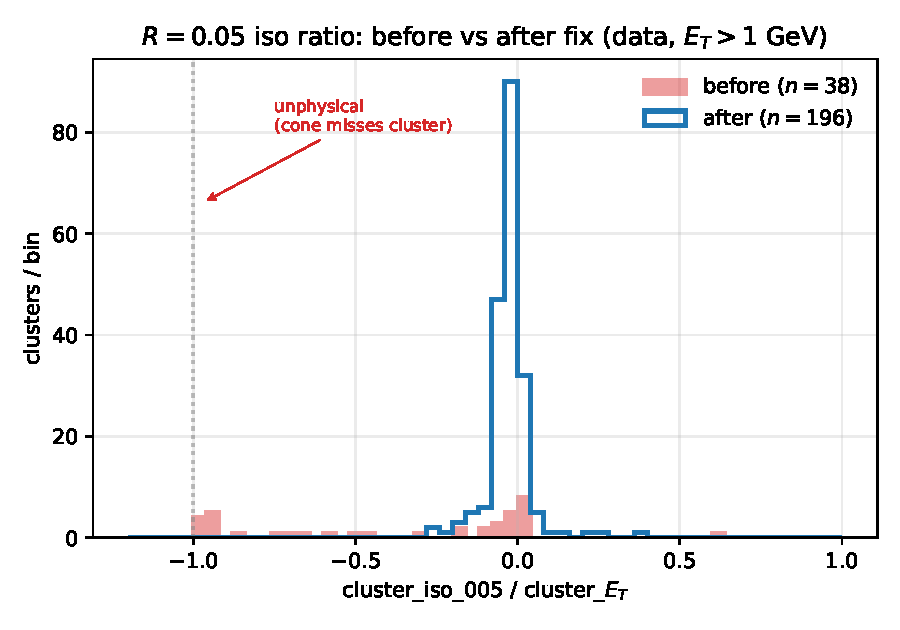
\includegraphics[width=0.68\linewidth]{figures/iso_cone_fix/iso005_ratio_1d.pdf}
  \caption{Distribution of \branch{cluster\_iso\_005}\,/\,\mbox{cluster\_$E_T$}
           in Run\,24 data ($E_T > 1$\,GeV). The pile-up at $-1$ (before fix,
           red) is the fingerprint of the cone geometrically missing the
           cluster itself. After fix (blue) the distribution is physical, with
           no population near $-1$.}
  \label{fig:iso005_1d}
\end{figure}

\subsection{$|v_z|$-correlation identified the depth mismatch}

The smoking gun was that the pathology is strongly correlated with the primary
vertex position. Figure~\ref{fig:iso005_vs_vz} plots the ratio against
$|v_z|$: before the fix, clusters at $|v_z| > 60$\,cm drive straight to the
unphysical $-1$ line, while low-$|v_z|$ clusters are healthy. After the fix,
the ratio is flat in $|v_z|$.

\begin{figure}[H]
  \centering
  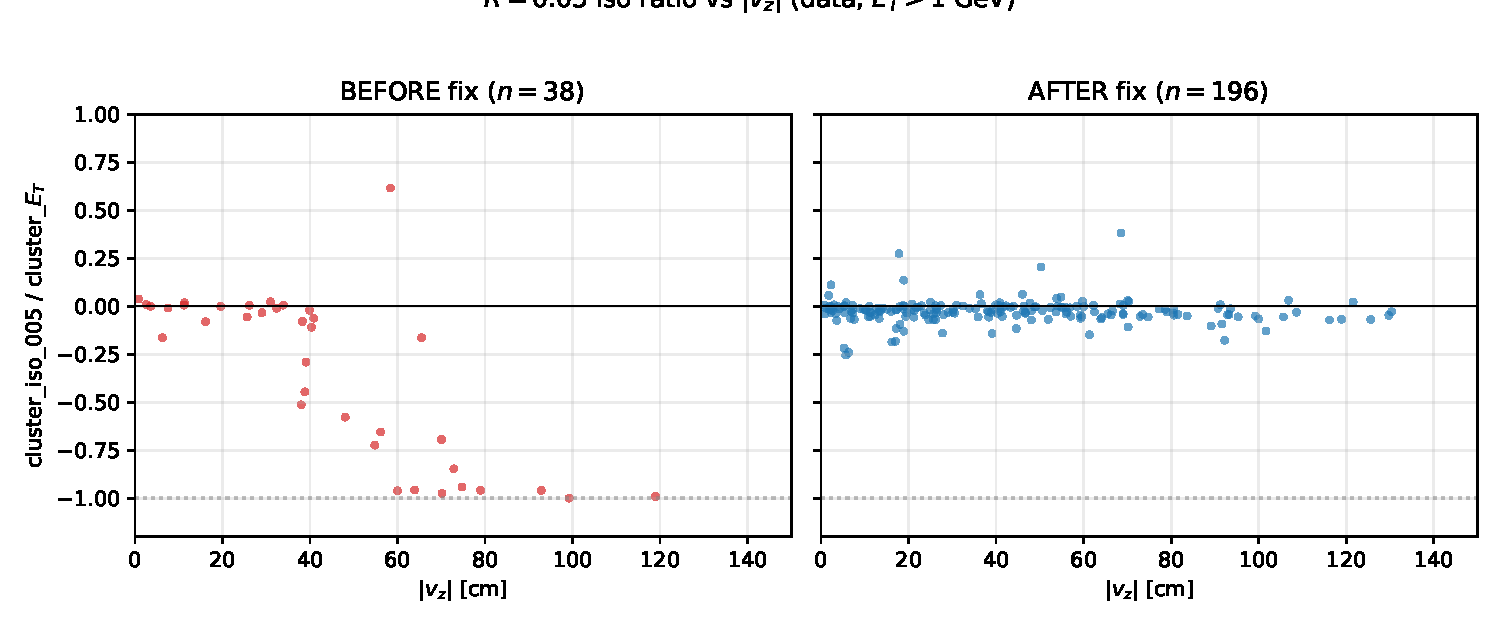
\includegraphics[width=\linewidth]{figures/iso_cone_fix/iso005_vs_vz.pdf}
  \caption{\branch{cluster\_iso\_005}\,/\,cluster\_$E_T$ vs.\ $|v_z|$ before
           (left, red) and after (right, blue) the fix. The pre-fix trend
           towards $-1$ at large $|v_z|$ is the $\sim |v_z|/R$ depth-mismatch
           signature; it is absent after the fix.}
  \label{fig:iso005_vs_vz}
\end{figure}

The pathological rate binned in $|v_z|$ makes the transition sharp
(Fig.~\ref{fig:pathol_vs_vz}). Before the fix the fraction of clusters with
\branch{iso\_005} $\approx -E_T$ goes from 0\,\% below $|v_z| = 40$\,cm to
100\,\% above 80\,cm; after the fix it is consistent with zero everywhere.

\begin{figure}[H]
  \centering
  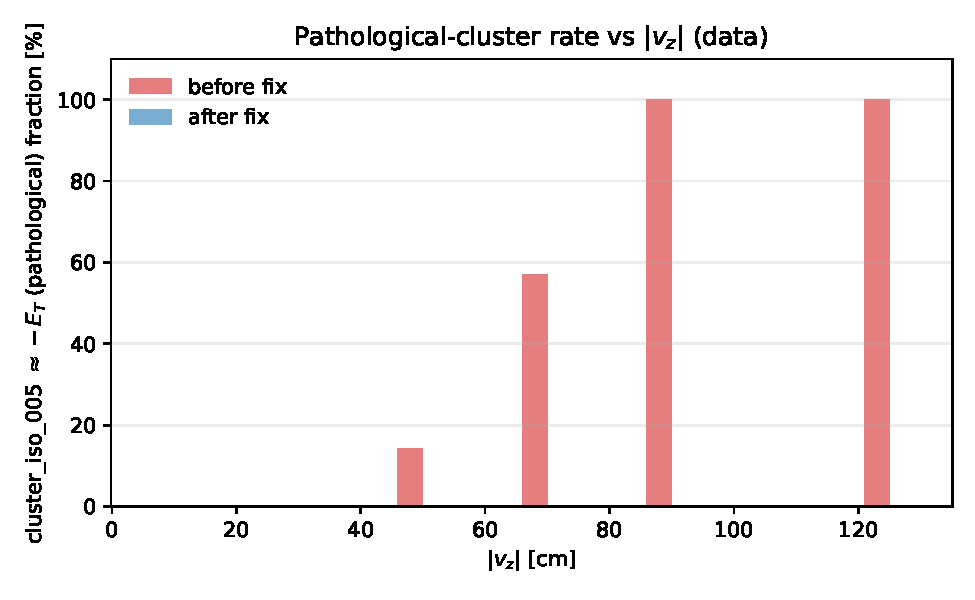
\includegraphics[width=0.68\linewidth]{figures/iso_cone_fix/pathological_vs_vz.pdf}
  \caption{Fraction of clusters with \branch{cluster\_iso\_005} $\in [-1.1, -0.9]\,E_T$
           (``pathological''), binned in $|v_z|$.}
  \label{fig:pathol_vs_vz}
\end{figure}

\subsection{Monotonicity cascade}

A photon cluster's isolation sum should be a non-decreasing function of cone
radius. Plotting \branch{iso}($R$)\,/\,cluster\_$E_T$ for each cluster as a
line in $R$, the pre-fix sample shows many lines that start at $-1$ (cone at
$R = 0.05$ captures nothing) and climb back to 0 as $R$ grows enough to
re-contain the cluster -- a textbook mis-centering signature. Post-fix the
ensemble is monotone and small, as expected (Fig.~\ref{fig:cascade}).

\begin{figure}[H]
  \centering
  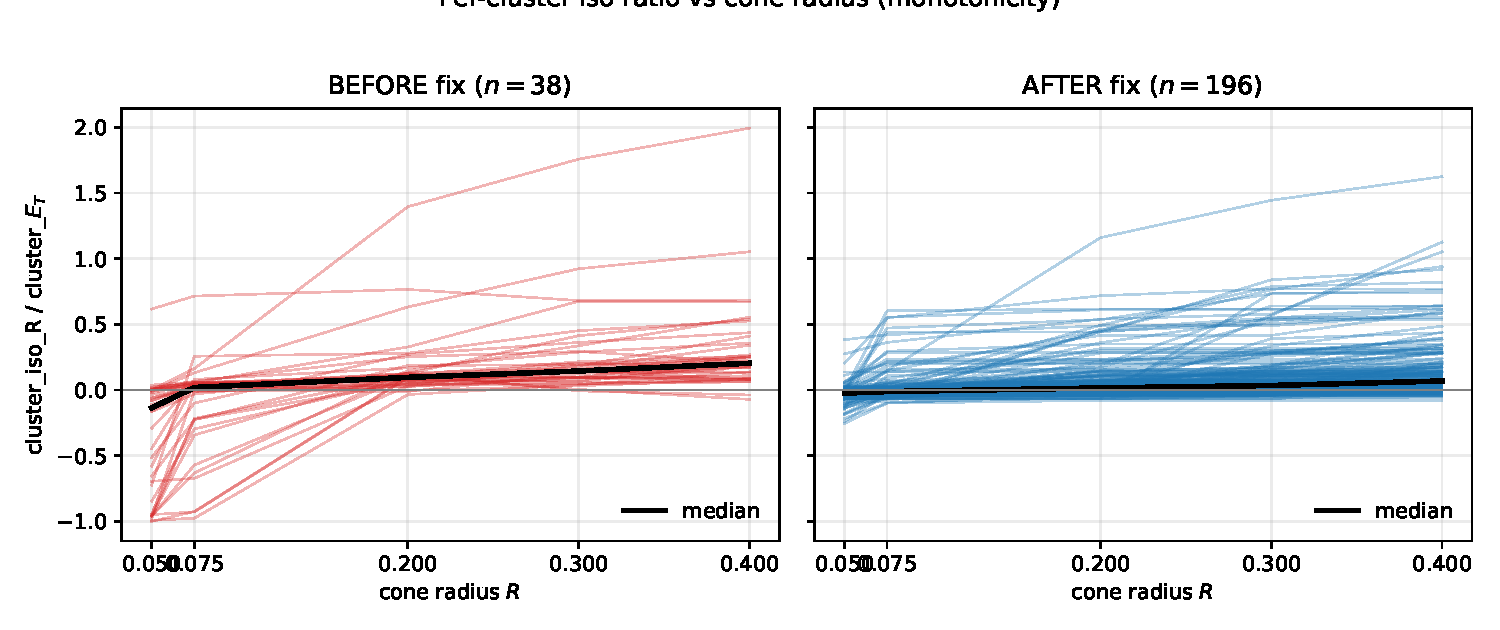
\includegraphics[width=\linewidth]{figures/iso_cone_fix/iso_cascade.pdf}
  \caption{Per-cluster \branch{iso}($R$)\,/\,cluster\_$E_T$ vs.\ cone radius.
           Black line: median over all clusters. Before fix (left): many
           clusters have $\text{iso}(R=0.05) \ll 0$, walking back to zero as
           $R$ grows past the mis-centering offset. After fix (right):
           monotone and bounded, as required.}
  \label{fig:cascade}
\end{figure}

\section{Root cause}

\begin{description}
  \item[Cone axis.] Line 1180 of \branch{CaloAna24.cc} set
    \verb|eta = RawClusterUtility::GetPseudorapidity(*recoCluster, vertex)|,
    which projects \verb|recoCluster->get_position()| through
    \verb|vertex = (0, 0, m_vertex)|. The sPHENIX cluster COG already has a
    shower-depth correction applied (the position sits at the energy-weighted
    \emph{shower} depth, $R_{\rm cluster} \approx 95$\,cm for a photon).
  \item[Constituent frame.] In \verb|calculateET| (tower iso) and
    \verb|calculateET_topo_6cones| (topo iso) each constituent's $\eta$ is
    obtained from \verb|RawTowerGeom::get_center_*| (tower geometric center,
    $R_{\rm tow} \approx 102$\,cm) or from the topo-cluster's energy-weighted
    cell centroid (also at tower mid-depth, and further out if HCal cells
    contribute).
  \item[Projected offset.] For a photon at physics $\eta_0$ and a vertex at
    $v_z$, the two paths project to
    \[
      \eta_{\rm axis} \;-\; \eta_{\rm const}
      \;\simeq\; v_z \, (\tfrac{1}{R_{\rm cluster}} - \tfrac{1}{R_{\rm tow}})
      \,\cosh\eta_0
      \,,
    \]
    which for $R_{\rm cluster} = 95$\,cm, $R_{\rm tow} = 102$\,cm, $v_z = 80$\,cm,
    $\eta_0 = 0.3$ gives $\Delta\eta \approx 0.05$ --- exactly at the edge of
    $R = 0.05$ and the threshold where the cluster's own central tower falls
    outside the cone. For $v_z = 100$\,cm the offset grows to $\approx 0.07$,
    producing a clean 100\,\% miss rate at $R = 0.05$.
\end{description}

Ownership exclusion was not the primary cause: the pathology affects the
topo-cluster path as well (which does not use identity-based self-exclusion
and has no per-tower threshold to toggle), with the same $|v_z|$-dependence.
That rules out the \verb|isGood| filter, the tower-container choice, and
the $-$cluster\_$E_T$ scalar subtraction as explanations on their own.

\section{Fix}

Three independent changes in \branch{CaloAna24.cc}, all on the same code path:

\begin{enumerate}
  \item \fix{CoG-tower axis.} Before the iso block, look up the central-tower
    geometry via
    \verb|RawTowerDefs::encode_towerid(CEMC, showershape[4], showershape[5])|
    and project through $v_z$ using \verb|getTowerEta(cog_tg, 0, 0, vertexz)|
    and \verb|cog_tg->get_phi()|. These values, \verb|iso_axis_eta| and
    \verb|iso_axis_phi|, are passed to every \verb|calculateET(...)| and
    \verb|calculateET_topo_6cones(...)| call. Cone axis and constituents now
    live on the same reference surface; the $|v_z|$-dependent offset cancels.
  \item \fix{Ownership-excluded variant.} A new helper
    \verb|calculateET_excl(eta, phi, dR, layer, min_E, skip_towerinfo_keys)|
    mirrors \verb|calculateET| but skips towers whose
    \verb|TowerInfoDefs::encode_emcal| key is in the skip set. The set is
    built from \verb|recoCluster->get_towermap()| for each cluster. Six new
    branches \branch{cluster\_iso\_excl\_\{005, 0075, 01, 02, 03, 04\}} are
    written as \(\sum_{\rm layers}\) without the scalar
    $-$cluster\_$E_T$ subtraction.
  \item \fix{Unified 120 MeV tower threshold.} All manual full-calo iso
    branches (\branch{cluster\_iso\_\{005, 0075, 02, 03, 04\}} and
    \branch{cluster\_iso\_excl\_*}) use \verb|min_E = 0.12|\,GeV. The built-in
    \verb|RawCluster::get_et_iso(2+i, false, true)| accessor (no threshold,
    cluster-COG axis) is no longer read; its previous consumers
    \branch{cluster\_iso\_\{02, 03, 04\}} are replaced by manual sums.
    Per-layer $60 / 70 / 120$\,MeV families are unchanged.
\end{enumerate}

The header (\branch{CaloAna24.h}) gains \verb|#include <set>|, the six
\verb|cluster_iso_excl_*| data members, and the \verb|calculateET_excl|
declaration.

\section{Verification}

\subsection{Before/after on data}

Table~\ref{tab:before_after} summarizes the pathological rates binned in
$|v_z|$. The pre-fix numbers come from a slimtree produced by the committed
HEAD before this change; the post-fix numbers come from re-running the same
anatreemaker macro with the fix applied.

\begin{table}[H]
  \centering
  \caption{Pathological-cluster fraction (\texttt{cluster\_iso\_005}
           $\in [-1.1, -0.9]\,E_T$) in Run~24 data
           (run 47289, segment 0, $E_T > 1$\,GeV).}
  \label{tab:before_after}
  \begin{tabular}{lrrrr}
    \toprule
    $|v_z|$ bin & $n_{\rm before}$ & pathol before & $n_{\rm after}$ & pathol after \\
    \midrule
    $0 - 40$\,cm    &  20 &   \phantom{00}0.0\,\% & 103 & \fix{0.0\,\%} \\
    $40 - 80$\,cm   &  14 &   \phantom{0}35.7\,\% &  65 & \fix{0.0\,\%} \\
    $80+$\,cm       &   4 & \crit{100.0\,\%}      &  28 & \fix{0.0\,\%} \\
    \midrule
    \textbf{all}    &  \textbf{38} & \crit{\textbf{23.7\,\%}} & \textbf{196} & \fix{\textbf{0.0\,\%}} \\
    \bottomrule
  \end{tabular}
\end{table}

Per-cluster monotonicity is also restored: post-fix, 100\,\% of clusters satisfy
$\text{iso}_{005} \le \text{iso}_{02} \le \text{iso}_{04}$ (within a 1\,MeV
rounding slop), against frequent violations pre-fix.

\subsection{New \texttt{iso\_excl} family}

The \branch{cluster\_iso\_excl\_*} branches are now the preferred small-$R$
iso measure: the cone axis is on the correct frame, the cluster's own
towers are removed by identity, and there is no scalar-$E_T$ subtraction that
could drive the value unphysically negative. Figure~\ref{fig:excl} shows the
post-fix distributions in data: non-negative populations growing with cone
radius, as expected for a pure neighbor-energy isolation.

\begin{figure}[H]
  \centering
  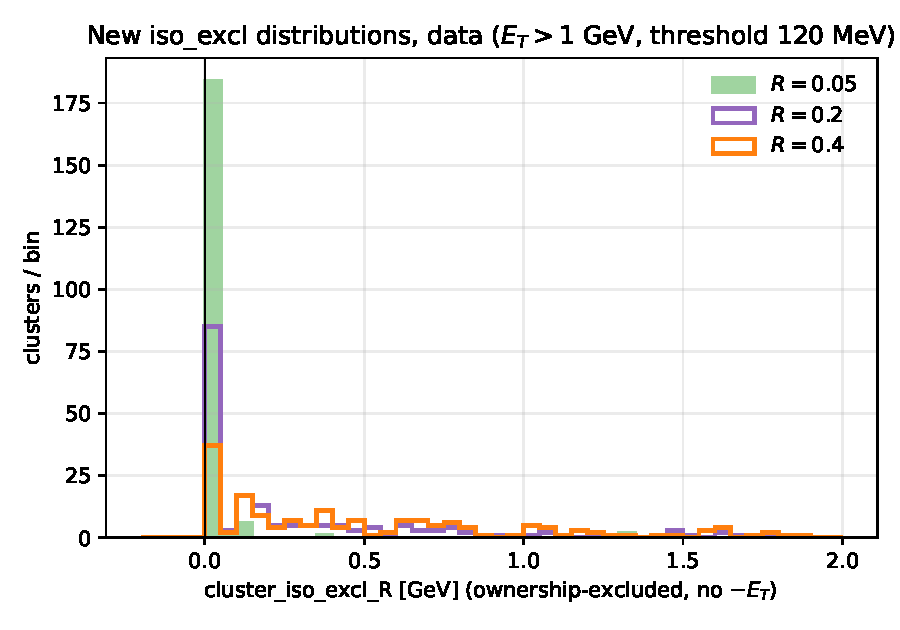
\includegraphics[width=0.72\linewidth]{figures/iso_cone_fix/iso_excl_distributions.pdf}
  \caption{Post-fix \branch{cluster\_iso\_excl\_R} distributions at $R = 0.05$,
           $0.2$, $0.4$ (data, $E_T > 1$\,GeV, 120\,MeV tower threshold).}
  \label{fig:excl}
\end{figure}

\section{Downstream implications}

\begin{itemize}
  \item The nominal PPG12 isolation selection is on
    \branch{cluster\_iso\_topo\_04} with
    \verb|reco_iso_max = reco_iso_max_b + reco_iso_max_s * ET| (parametric cut
    in the efficiency configs). The topo path gets the same CoG-tower-axis
    fix; the $|v_z|$-dependent tail is removed. For low-$|v_z|$ clusters the
    nominal iso is essentially unchanged. For high-$|v_z|$ clusters, pre-fix
    values that had been artificially pushed toward $-E_T$ now sit at the
    physical value, so those clusters migrate from
    $\text{noniso}$ into $\text{iso}$ of the ABCD regions (affects
    $A, B, C, D$ populations and consequently purity and efficiency).
  \item \branch{cluster\_iso\_\{02, 03, 04\}} now come from the manual
    120\,MeV-threshold path rather than the built-in
    \verb|get_et_iso| (no threshold, cluster-COG axis). Downstream code that
    reads these branches (e.g.\ \branch{efficiencytool/*.C},
    \branch{FunWithxgboost/apply\_BDT.C}, \branch{BDTinput.C}) will see
    numerically different values even for low-$|v_z|$ clusters --- the
    threshold change alone shifts the iso scale. The parametric iso cut
    (\verb|reco_iso_max_b|, \verb|reco_iso_max_s|) may need retuning on the
    new distribution.
  \item Production of fresh slimtrees is required before any downstream
    efficiency / purity / cross-section re-run. The fix is committed on
    \texttt{main} at \texttt{89941f1} (anatreemaker).
\end{itemize}

\section*{Files}

\begin{itemize}
  \item \branch{anatreemaker/source/CaloAna24.cc} --- cone-axis replacement
    (L1207--1246), per-layer 120\,MeV sums for $R = 0.1, 0.2, 0.4$
    (L1291--1302), \branch{\_excl} callers (L1303--1308),
    \branch{iso\_02/03/04} manual fills (L1862--1864),
    \branch{iso\_excl} branch writes (L1884--1890),
    \branch{calculateET\_excl} implementation (L2447--2518).
  \item \branch{anatreemaker/source/CaloAna24.h} --- \branch{<set>} include,
    six \branch{cluster\_iso\_excl\_*} data members,
    \branch{calculateET\_excl} declaration.
  \item \branch{reports/figures/iso\_cone\_fix/make\_plots.py} --- diagnostic
    script that reproduces every figure in this note from the two
    slimtree test outputs.
\end{itemize}

\end{document}
